\documentclass[12pt,a4paper]{article}
\usepackage[left=10mm,right=10mm,top=20mm,bottom=20mm]{geometry}
\usepackage{amsmath}
\usepackage{physics}
\newcommand{\dbar}{d\hspace*{-0.08em}\bar{}\hspace*{0.1em}}
\usepackage{shapepar}
\usepackage{multicol}
\usepackage{MnSymbol}
\usepackage{color}
\usepackage{enumitem}
\usepackage{siunitx}
\usepackage{tikz}
\usepackage{pgfplots}
\usepackage{makecell}
\usepackage{graphicx}
\usepackage{gensymb}
\usepackage{caption}
\usepackage{hyperref}
\usepackage{multirow}
\usepackage{mathtools}
\usepackage{esdiff}
\usepackage{subfigure}

\title{Data Analysis on Long Period Variable Stars Using Gaia Data}
\author{Hossein Mahdaei and Mohammad Jamshidi}
\date{}
\begin{document}
	\maketitle
	\section*{Introduction to Gaia}
	Gaia is a space observatory of the European Space Agency (ESA), launched in 2013 and expected to operate until 2025. The spacecraft is designed for astrometry: measuring the positions, distances and motions of stars with unprecedented precision. The mission aims to construct by far the largest and most precise 3D space catalog ever made, totalling approximately 1 billion astronomical objects, mainly stars, but also planets, comets, asteroids and quasars, among others.
	
	The successor to the Hipparcos mission (operational 1989–1993), Gaia is part of ESA's Horizon 2000+ long-term scientific program. Gaia was launched on 19 December 2013 by Arianespace using a Soyuz ST-B/Fregat-MT rocket flying from Kourou in French Guiana. The spacecraft currently operates in a Lissajous orbit around the Sun–Earth L2 Lagrangian point. 
	\begin{figure}[ht]
		\centering
		\caption{Artist's impression of the Gaia spacecraft.}
		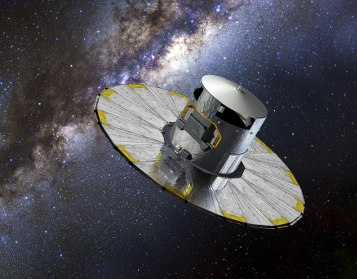
\includegraphics[width=0.7\linewidth]{gaia.png}
	\end{figure}	
	Gaia has these goals: Determine the position, parallax and annual proper motion of 1 billion stars with an accuracy of about 20 microarcseconds (μas) at 15 mag, and 200 μas at 20 mag. Determine the positions of stars at a magnitude of V = 10 down to a precision of 7 μas—this is equivalent to measuring the position to within the diameter of a hair from 1000 km away—between 12 and 25 μas down to V = 15, and between 100 and 300 μas to V = 20, depending on the colour of the star. The distance to about 20 million stars will thus be measured with a precision of 1\% or better, and about 200 million distances will be measured to better than 10\%. Distances accurate to 10\% will be achieved as far away as the Galactic Centre, 30,000 light-years away. Measure the tangential speed of 40 million stars to a precision of better than 0.5 km/s. Derive the atmospheric parameters (effective temperature, line-of-sight interstellar extinction, surface gravity, metallicity) for all stars observed, plus some more detailed chemical abundances for targets brighter than V = 15. Measure the orbits and inclinations of a thousand extrasolar planets accurately, determining their true mass using astrometric planet detection methods. More precisely measure the bending of starlight by the Sun's gravitational field, predicted by Albert Einstein's General Theory of Relativity and first detected by Arthur Eddington during a 1919 solar eclipse, and therefore directly observe the structure of spacetime. Potential to discover Apohele asteroids with orbits that lie between Earth and the Sun, a region that is difficult for Earth-based telescopes to monitor since this region is only visible in the sky during or near the daytime. Detect up to 500,000 quasars.
	
	The total cost of the mission is around €740 million (about 1 billion dolor), including the manufacture, launch and ground operations.
	
	\section*{Intdocuntion to Long-Period Variable Stars}
	
	The descriptive term long-period variable star refers to various groups of cool luminous pulsating variable stars. It is frequently abbreviated to LPV.
	
	Long period variables are pulsating cool giant, or supergiant, variable stars with periods from around a hundred days, or just a few days for OSARGs, to more than a thousand days. In some cases, the variations are too poorly defined to identify a period, although it is an open question whether they are truly non-periodic.
	\begin{figure}[ht]
		\centering
		\caption{A cluster that is observed by Gaia.}
		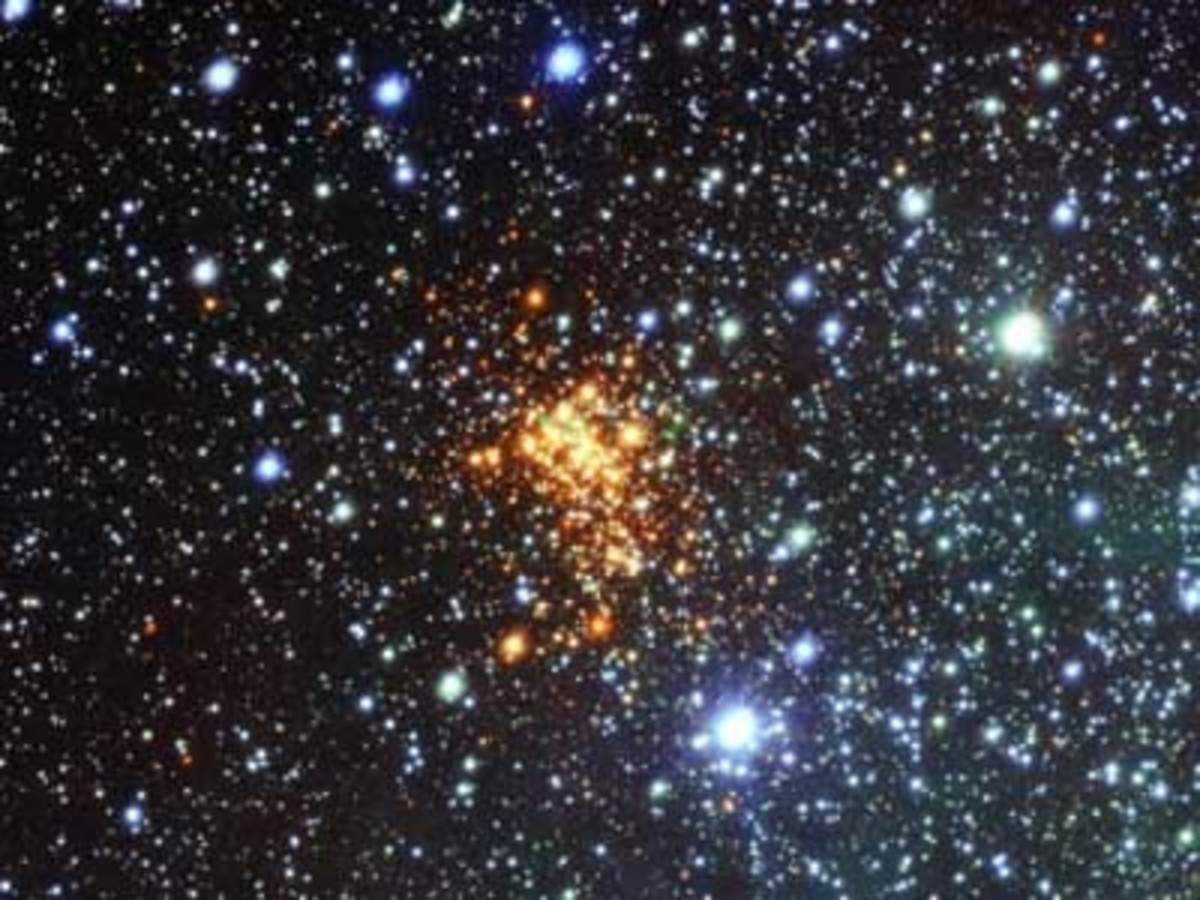
\includegraphics[width=0.7\linewidth]{cluster.png}
	\end{figure}
	LPVs have spectral class F and redwards, but most are spectral class M, S or C. Many of the reddest stars in the sky, such as Y CVn, V Aql, and VX Sgr are LPVs.
	
	\section*{Diagrams and Data}
	Here we represent our diagrams that made using Gaia data (\url{https://cdn.gea.esac.esa.int/Gaia/gdr2/vari_long_period_variable/csv/}).
	\begin{figure}[ht]
		\centering
		\caption{Visible absolute magnitude per logarithm of the period.}
		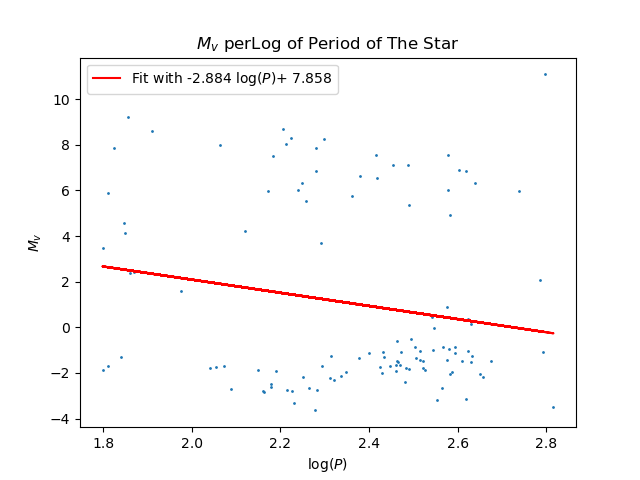
\includegraphics[width=0.6\linewidth]{Mv_s_per_log(P).png}
	\end{figure}

	\begin{figure}[ht]
		\centering
		\caption{Histogram distribution of periods.}
		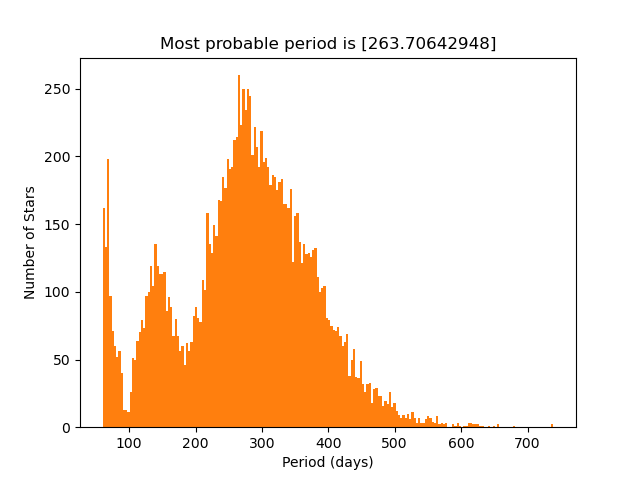
\includegraphics[width=0.6\linewidth]{P_s_disturb.png}
	\end{figure}

	\begin{figure}[ht]
		\centering
		\caption{Distribution of red supergiants and non-red supergiants.}
		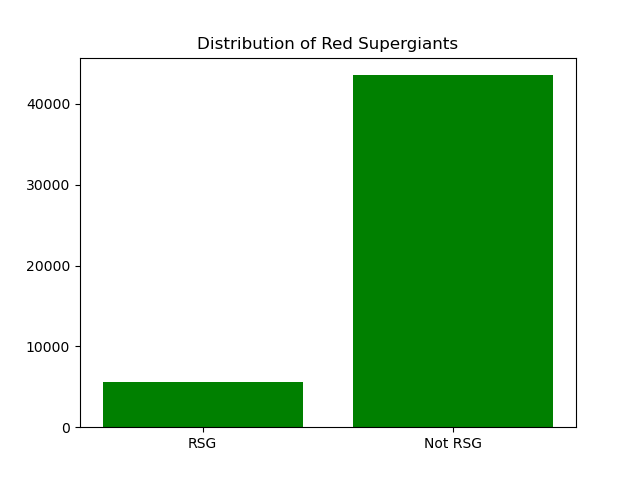
\includegraphics[width=0.6\linewidth]{rsg_disturb.png}
	\end{figure}	

\newpage
\section*{Resources}
1. \url{https://en.wikipedia.org/wiki/Gaia_(spacecraft)}
\newline
2. \url{https://en.wikipedia.org/wiki/Long-period_variable_star}
\newline
3. \url{https://cdn.gea.esac.esa.int/Gaia/gdr2/vari_long_period_variable/}
\newline
4. Lecture notes of the course (Astrophysics Course, Spring 2022, Dr. Bahmanabadi)
\end{document}


